\section{Methods}
\vspace{-.2cm}
In this section, we will describe the PH-Reg framework, which we illustrate in Figure~\ref{fig:arch}. This framework enables \emph{existing pretrained ViTs} to benefit from register tokens, yielding significantly cleaner dense representations. During training, PH-Reg requires only unlabeled images for the self-distillation process. In section~\ref{teacher_method}, we will first describe the denoising process of teacher network outputs. Unlike prior work that rely on a neural field/hash-grid, this method denoises dense features without the use of expensive gradient-based learning. In section~\ref{student_method}, we will describe how we initialize and modify the student architecture. This approach only introduces a small set of additional parameters to the network. Finally in section~\ref{learning_method} we will describe our distillation process. 

\begin{figure}[t]
  \centering
  \vspace{-2em}
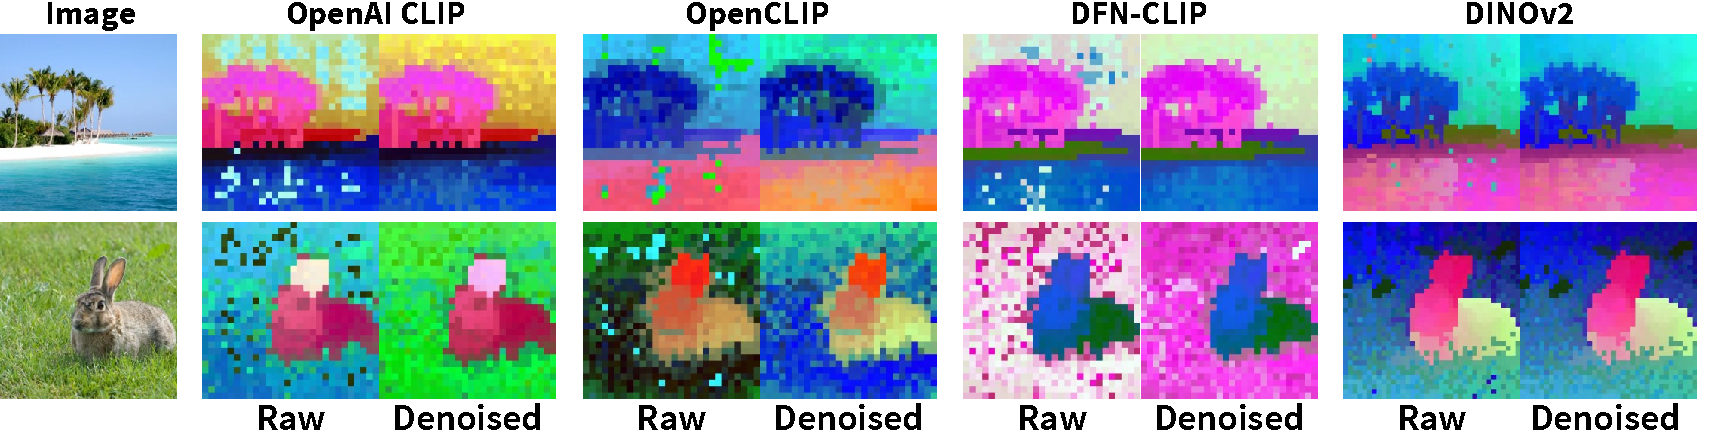
\includegraphics[width=1.0\linewidth]{fig_pdf/denoise.pdf}
  \caption{\textbf{Denoising Teacher Representations with Augmentations.} For each model, we visualize the UMAP of dense features before and after applying test-time augmentation. The results show that our proposed method produces noticeably cleaner dense feature representations without requiring gradient-based learning. Please zoom in for details.}
  \vspace{-.5cm}
  \label{fig:denoise}
\end{figure}

\vspace{-.2cm}
\subsection{Efficient Denoising of Teacher Representations}
\label{teacher_method}
\vspace{-.2cm}

\renewcommand{\figurename}{Algorithm}
\begin{wrapfigure}{r}{0.46\textwidth}
\vspace{-0.5em}
\begin{minipage}{1.0\linewidth}
  \begin{algorithm}[H]
  \caption{\textbf{Denoising Process}}
  \label{distill_algo}
    \textbf{Input:} Image $\mathcal{I}\in\mathbb{R}^{H\times W \times 3}$;\\
    \hspace{10.7mm}Image space coordinates $\mathcal{C}\in [0,1] \times [0,1]$;\\
    \hspace{10.7mm}Augmentation parameters $\theta_{1}, \theta_{2},..., \theta_{n}$;\\ 
    \hspace{10.7mm}Augmentation function $\mathcal{T}$;\\
    \hspace{10.7mm}ViT teacher model $f_{teacher}$; 
\\
1. Zero init clean feature tensor $Q$\\
2. Zero init count tensor $K$\\
3. \textbf{For} i in \{1, ..., n\}:\\
4. \hspace{6.0mm} $\theta_i =(x_i, y_i, \text{flip}_i)$ 
\\
5. \hspace{6.0mm} $(\mathcal{I}_i,\mathcal{C}_i) = \mathcal{T}(\mathcal{I}, \mathcal{C}, \theta_i)$\\
6. \hspace{6.0mm} Dense feature $F_i = f_{teacher}(\mathcal{I}_i)$\\
7. \hspace{6.0mm}$(F^\text{valid}_i,\mathcal{C}^\text{valid}_i) = \mathcal{T}^{-1}(F_i, \mathcal{C}_i, \theta_i)$\\
8. \hspace{6.0mm}$Q[\mathcal{C}^\text{valid}_i]=Q[\mathcal{C}^\text{valid}_i]+F^\text{valid}_i$\\
9. \hspace{6.0mm}$K[\mathcal{C}^\text{valid}_i]=K[\mathcal{C}^\text{valid}_i]+1$\\
10. \textbf{return} $Q/K$
  \end{algorithm}
\end{minipage}\vspace{-0.1em}
\end{wrapfigure}
\vspace{-0.5em}
\renewcommand{\figurename}{Figure}

Our denoising process starts from the observation that artifact tokens are not static relative to image content. Put another way, if an image is shifted by a certain amount (with the gaps padded with whitespace), the artifacts do not shift by the same amount. As shown in Figure~\ref{fig:arch}, given an RGB image $\mathcal{I}\in\mathbb{R}^{H\times W \times 3}$, we randomly sample $n$ random augmentation parameters $(\theta_1, \theta_2, ...,\theta_n)$, where each $\theta_i$ defines a horizontal/vertical offset $(x_i,y_i)$ and boolean $\text{flip}_i \in \{0,1\}$ defined horizontally. For each image, we also compute the image space coordinate grid $\mathcal{C} = (\text{x-coords},\text{y-coords})$. Where $(x,y)$ are respectively in range $[0,1]$: $x$ defines the left-right axis, and $y$ defines the top-down axis. The coordinates $\mathcal{C}$ help us keep track of the original location of an image region after augmentation. In practice, as we are working with a ViT model with patch size $k\times k$, where the tokenization process yields a $(\frac{H}{k},\frac{W}{k})$ grid of image tokens, we define our parameters using offsets that are integer multiples of $k$ to facilitate efficient indexing.
Together, the image $\mathcal{I}$, the coordinates $\mathcal{C}$, and augmentation parameter $\theta_i$ are provided to transform function to yield an augmented image $\mathcal{I}_i$ and new coordinates $\mathcal{C}_i$: $\mathcal{T}(\mathcal{I}, \mathcal{C},\theta_i) \Rightarrow (\mathcal{I}_i,\mathcal{C}_i)$. 

% \setcounter{figure}{3} 
\begin{figure}[t]
  \centering
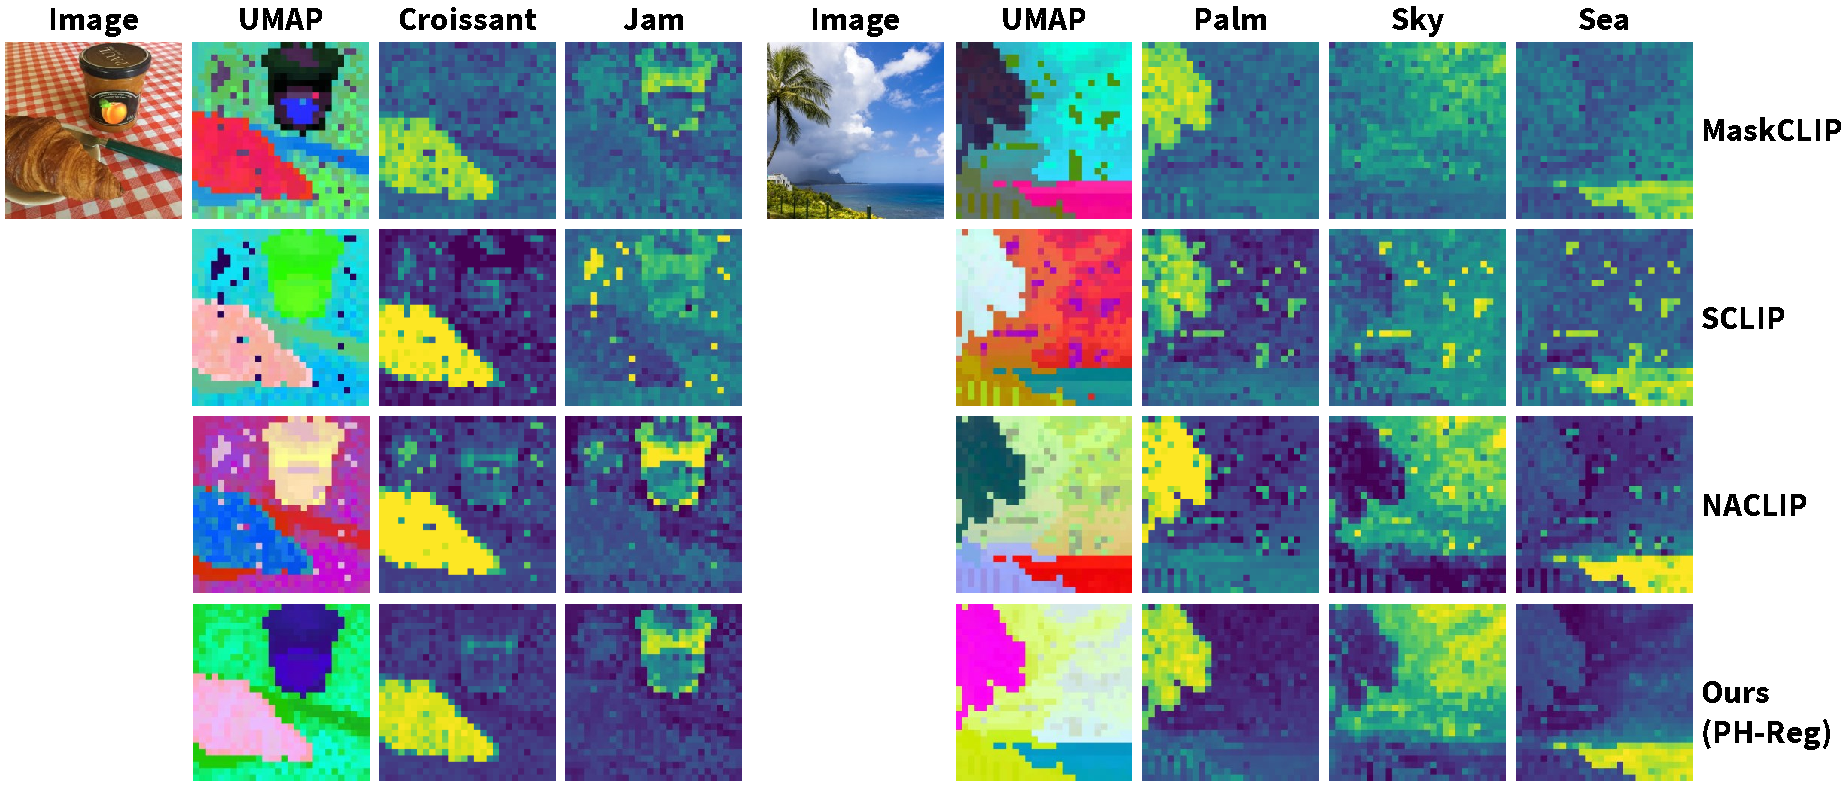
\includegraphics[width=1.0\linewidth]{fig_pdf/similarityfinal.pdf}
   \vspace{-5mm}
  \caption{\textbf{Visualization of Open-vocabulary Semantic Segmentation.}  We compare against MaskCLIP, SCLIP, NACLIP, and find that our method yields clean feature maps free of artifacts.}
  \vspace{-0.2em}
  \label{fig:local}
\end{figure}

A teacher model $f_\text{teacher}$ is based on a frozen set of original network weights, without any additional parameters. Given an augmented image $\mathcal{I}_i$, this network outputs feature $F_i$. We restore the features to the original location within an image using the inverse transform function $\mathcal{T}^{-1}(F_i, \mathcal{C}_i)$. The restored features are additively accumulated across different augmentation parameters, while keeping track of the number of occurrences for each location. At the end, the dimension-wise sample mean is computed for the accumulated features. We present our full denoising process in Algorithm~\ref{distill_algo}.
The patch-wise expected value of this representation is the same as the optimal value when optimizing a discrete grid of representations to minimize mean squared error (as used in DVT~\citep{yang2024denoising} and traditional neural field based methods). However, as we do not require gradients, this denoising process can be done in less than \textit{200ms}, roughly two magnitudes faster than neural field based denoising in DVT. The comparison between raw and denoised dense feature visualizations is shown in Figure~\ref{fig:denoise}.


\vspace{-.2cm}
\subsection{Design of the Student Network}
\label{student_method}
\vspace{-.2cm}
Our objective is to preserve maximimal computational efficiency of the student model, while leveraging the knowledge of the pre-trained weights. For this purpose we introduce $m$ number of register tokens, providing a minimally invasive enhancement to the base architecture. After the addition of register tokens, a total of $m + 1 + \frac{H}{k} \times \frac{W}{k}$ tokens participate in the self-attention process. Unlike prior work that trains registers from scratch~\citep{darcet2023vision}, this approach updates only these registers and selectively unfreezes specific components during distillation, preserving the majority of the ViT’s pretrained weights. Through ablation studies, we identify optimal unfreezing strategies, such as adjusting convolution layers, positional embeddings, or the last transformer block. 
\vspace{-.2cm}
\subsection{Learning and Optimization of the Student}
\label{learning_method}
\vspace{-.2cm}
We employ a multi-objective distillation strategy, combining cosine similarity and mean squared error losses to ensure both directional and magnitude alignment between teacher representations $F_{teacher}$ and student representations $F_{student}$. Our final loss is: $\text{Loss}_{\text{total}} = \text{1} -\texttt{cossim}(\text{target}, \text{predicted}) + \texttt{MSE}(\text{target}, \text{predicted})$.
